\chapter{Análisis de resultados}
\label{chap:analisis}

\section{Análisis de los resultados obtenidos con \emph{Lenna}}\label{sect:arimg}

    A continuación, se presenta un análisis comparativo entre todas las
metaheurísticas hibridas implementadas (\emph{GAH}, \emph{NPSOH}, \emph{WPSOH},
\emph{NDEH}, \emph{SDEH}, \emph{BeeH} y \emph{AntH}) y el algoritmo determinista
\emph{K-means}. Las metaheurísticas híbridas fueron elegidas para este análisis
por presentar mejor calidad en sus soluciones finales que las metaheurísticas no
híbridas (véase el apéndice \ref{apendicec}).

    Los datos utilizados provienen de los resultados obtenidos con el mejor
conjunto de valores encontrado para cada metaheurística con la imagen
\textbf{Lenna} (ver sección \ref{sect:impresultados} y apéndice \ref{apendicea}).

\subsection{Comparación por calidad de solución final: índice $DB$}\label{analisis:db}

    Como se mencionó en la sección \ref{sect:tval}, el índice $DB$ mide la
calidad de una partición en función de las distancias \emph{intra-cluster} e
\emph{inter-cluster}. Mientras menor sea el valor de este índice, se tiene mejor
calidad de partición.

\subsubsection{Prueba de diferencia de medias}\label{analisis:db_mean_hip}

    Para determinar diferencias en la calidad de las soluciones finales de los
algoritmos implementados y elegir al mejor de todos, se realizó una prueba de
hipótesis de diferencia de medias para el índice $DB$. Se debe probar para
cada par de algoritmos $i, j \in Algorithms \land i \neq j$ alguna de las
siguientes hipótesis:
\begin{itemize}
    \item \emph{Hipótesis nula}: $\bar{X}_i - \bar{X}_j = 0$
    \item \emph{Hipótesis altenativa}: $\bar{X}_i - \bar{X}_j \neq 0$
\end{itemize}
donde
\begin{itemize}
    \item $\bar{X}_i$ es la media de las observaciones del valor del índice $DB$
          para el algoritmo $i$.
    \item $Algorithms$ es el conjunto de grupos a estudiar. Está conformado por
los algoritmos implementados: \{\emph{K-means}, \emph{GAH}, \emph{NPSOH},
\emph{WPSOH}, \emph{NDEH}, \emph{SDEH}, \emph{BeeH}, \emph{AntH}\}.
\end{itemize}

\subsubsection{Prueba de diferencia de varianzas}\label{analisis:db_var_hip}

    Para determinar el estadístico de la prueba descrita en la sección
anterior (ver sección \ref{analisis:db_mean_hip}) es necesario saber si las
observaciones de los valores del índice $DB$ de los diferentes algoritmos
presentan homocedasticidad o heterocedasticidad (igual o diferente varianza
respectivamente). Fue elegida la prueba de \emph{Levene} \cite{Levene_Test}
debido a que permite la comparación de multiples grupos al mismo tiempo. Para
esta prueba se debe probar alguna de las siguientes hipótesis:
\begin{itemize}
    \item \emph{Hipótesis nula}: $\sigma_1 = \sigma_2 = \cdots = \sigma_i = \cdots = \sigma_n$
    \item \emph{Hipótesis alternativa}: al menos una de las varianzas es diferente.
\end{itemize}
donde $\sigma_i$ es la varianza poblacional del índice $DB$ para el algoritmo
$i$, $\forall i \in Algorithms$.

    El estadístico de la prueba de \emph{Levene} es el siguiente\cite{Levene_Test}:
\begin{equation}\label{levene_est}
    W = \displaystyle\frac{(N-k) \cdot \displaystyle\sum_{i = 1}^k N_i \cdot (Z_{i\cdot} - Z_{\cdot\cdot})^2}{(k - 1) \cdot \displaystyle\sum_{i = 1}^k \sum_{j = 1}^{N_i} (Z_{ij} - Z_{i\cdot})^2} \sim F_{\alpha, k - 1, N - k}
\end{equation}
donde
\begin{itemize}
    \item $k$ es la cantidad de grupos. Para efectos de esta prueba, es la
          cardinalidad del conjunto $Algorithms$.
    \item $N_i$ es el tamaño de la muestra para el algoritmo $i$.
    \item $N = \displaystyle\sum_{i \in Algorithms} N_i$
    \item $Y_{ij}$ es el $j$-ésimo valor de la muestra del algoritmo $i$.
    \item $Z_{ij} = |Y_{ij} - \tilde{Y}_i|$, donde $\tilde{Y}_i$
es la mediana de los valores de la muestra del algoritmo $i$.
    \item $Z_{\cdot\cdot} = \displaystyle\frac{1}{N} \displaystyle\sum_{i = 1}^k \sum_{j = 1}^{N_i} Z_{ij}$ es la media de todos los $Z_{ij}$.
    \item $Z_{i\cdot} = \displaystyle\sum_{j = 1}^{N_i} Z_{ij}$ es
la media del $Z_{ij}$ para el algoritmo $i$.
\end{itemize}

    Como se puede observar en el Resultado \ref{r_db_var_img} se rechaza la hipótesis
nula con un nivel de significancia menor a 5 \% (\emph{p-valor} $ = 6.025 \cdot 10^{-7}$).
Esto significa que existe una diferencia entre las varianzas de las muestras
del índice $DB$ de los algoritmos pertenecientes al conjunto $Algorithms$.
\textbf{Por lo tanto, las diferentes muestras presentan heterocedasticidad para
el índice $DB$}.

\begin{lstlisting}[float=h!, caption={Diferencia de Varianza: Índice \emph{DB}}, label=r_db_var_img]
> leveneTest(db, name)
Levene's Test for Homogeneity of Variance (center = median)
       Df F value    Pr(>F)    
group   7  6.4483 6.025e-07 ***
      231                      
---
Signif. codes:  0 '***' 0.001 '**' 0.01 '*' 0.05 '.' 0.1 ' ' 1 
\end{lstlisting}

\subsubsection{Intervalo de confianza de la prueba de diferencia de medias}\label{analisis:db_mean_est}

    En la sección anterior (ver sección \ref{analisis:db_var_hip}), se demostró
que las varianzas de las muestras del índice $DB$ de los algoritmos pertenecientes
al conjunto $Algorithms$ son diferentes. Por lo tanto, el estadístico de la prueba
de hipótesis descrita en la sección \ref{analisis:db_mean_hip} no debe ser
sensible a la varianza.

    Sobre los resultados se aplicó la prueba de \emph{Dunnett-Tukey-Kramer},
también llamada prueba \emph{T3} de \emph{Dunnett}, y fue elegida ya que
\cite{DTK_Test}:
\begin{itemize}
    \item No requiere que las varianzas de las muestras de los diferentes grupos
sean iguales.
    \item Permite la comparación de cada grupo con los demás sin aumentar la
probabilidad de cometer un error tipo I\footnote{Probabilidad de tener falsos
positivos}.
\end{itemize}

    El intervalo de confianza para la diferencia de medias de una prueba
\emph{T3} es el siguiente:
\begin{equation}\label{dtk_inter}
    \bar{X}_i - \bar{X}_j \pm q_{\alpha, k^{*}, \nu} \cdot \sqrt{\displaystyle\frac{S_{i}^2}{n_i} + \displaystyle\frac{S_{j}^2}{n_j}}
\end{equation}
donde
\begin{itemize}
    \item $\alpha$ es el nivel de confianza de la prueba.
    \item $\bar{X}_i - \bar{X}_j$ es la diferencia de medias del grupo $i$ con
el grupo $j$.
    \item $q$ es la distribución \emph{Studentized Range}.
    \item $i, j \in Algorithms$.
    \item $S_i$ es la varianza muestral del grupo $i$.
    \item $n_i$ es el tamaño de la muestra del grupo $i$.
    \item $k$ es la cantidad de grupos. Para efectos de esta prueba, es la
          cardinalidad del conjunto $Algorithms$.
    \item $k^{*}$ y $\nu$ son los grados de libertad del estadístico de la prueba:
          \begin{equation}
                k^{*} = \displaystyle\frac{k (k - 1)}{2}
          \end{equation}
          \begin{equation}\label{eq: nu}
            \nu = \displaystyle\frac{\left(\displaystyle\frac{S_{i}^2}{n_i} + \displaystyle\frac{S_{j}^2}{n_j}\right)^2}{\left(\displaystyle\frac{S_{i}^2}{n_i}\right)^2 \displaystyle\frac{1}{n_i - 1} + \left(\displaystyle\frac{S_{j}^2}{n_j}\right)^2 \displaystyle\frac{1}{n_j - 1}}
          \end{equation}
\end{itemize}

    En la figura \subref{fig:comp_inter} se pueden observar los intervalos de
confianza de la prueba \emph{T3} para el índice $DB$ de cada algoritmo comparado
con los demás. Los intervalos en rojo indican que existe una diferencia de calidad
de las soluciones finales de los algoritmos comparados con un nivel de significancia
de 5 \%. Por otro lado, los intervalos en negro indican que no existe una diferencia
de la calidad de las soluciones de los algoritmos comparados con un nivel de 
significancia de 5 \%. Por lo tanto, se puede concluir:
\begin{itemize}
    \item Los algoritmos \emph{K-means}, \emph{NPSOH}, \emph{WPSOH}, \emph{NDEH}
          y \emph{SDEH} tienen soluciones finales con calidad similar.
    \item Las metaheurísticas \emph{GAH} y \emph{BeeH} tienen soluciones finales
          con calidad similar y diferentes las de los demás algoritmos
          comparados.
    \item La calidad de las soluciones finales de la metaheurística \emph{AntH}
          es diferente a las calidades de las soluciones finales de los demás
          algoritmos.
\end{itemize}

    Tomando en cuenta el análisis anterior y el diagrama de cajas presentado en
la figura \subref{fig:comp_db}, se concluye:
\begin{itemize}
    \item Las metaheurísticas \emph{GAH} y \emph{BeeH} reportan los valores del
índice $DB$ promedio más bajo de todos los algoritmos comparados y, por lo tanto,
sus soluciones finales tienen mayor calidad que las de los demás algoritmos
implementados.
    \item La metaheurística \emph{AntH} reporta el valor del índice $DB$ promedio
más alto y, por lo tanto, sus soluciones finales tienen menor calidad que las de
los demás algoritmos implementados. Este comportamiento se puede observar con
claridad en en la figura \subref{fig:lennaant}, donde la imagen resultante
es difusa.
\end{itemize}

    \textbf{Así que las metaheurísticas cuyas soluciones finales tienen la mejor
calidad con respecto a las de los algoritmo implementados son \emph{GAH} y
\emph{BeeH}, ya que tienen los valores de índice $DB$ estadísticamente más bajos
(ver figuras \subref{fig:comp_db} y \subref{fig:comp_inter}).}

\begin{figure}[h!]
  \centering
  \subfloat[\emph{Diagramas de cajas del índice $DB$}]{\label{fig:comp_db}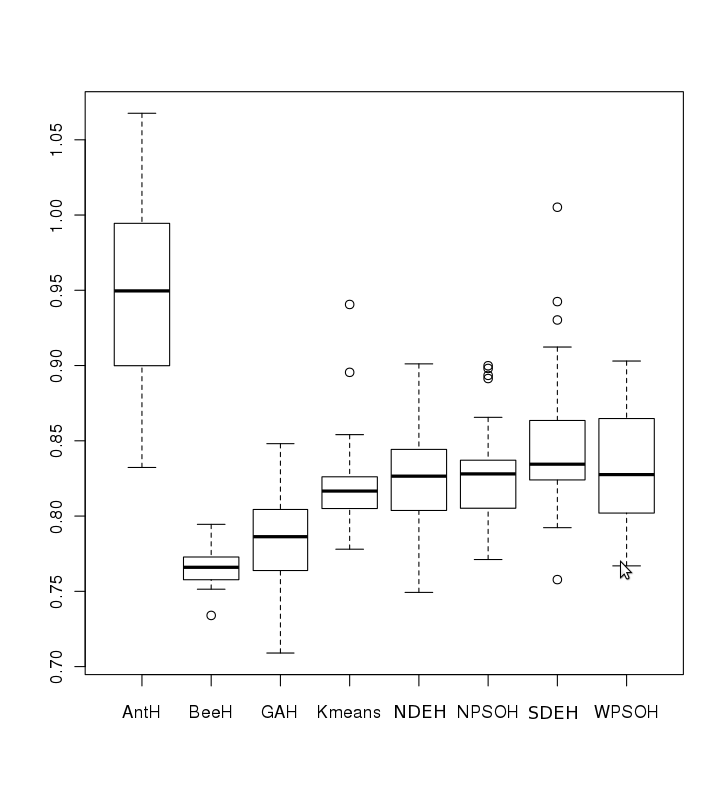
\includegraphics[width=0.6\textwidth]{figures/comp_db.png}}\\
  \subfloat[\emph{Intervalos de confianza del índice $DB$}]{\label{fig:comp_inter}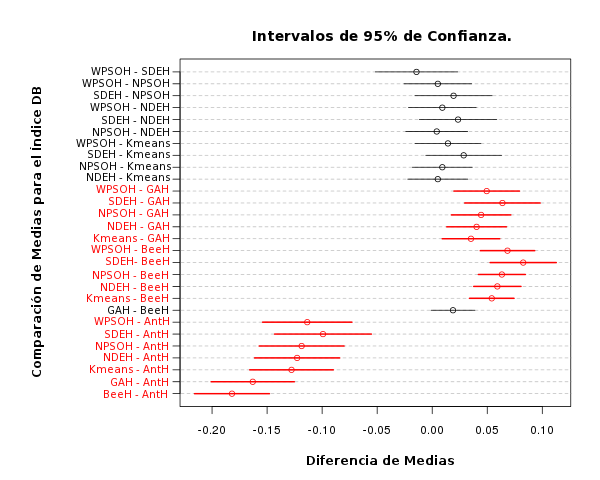
\includegraphics[width=0.6\textwidth]{figures/best_img_db.png}}
  \caption{Comparación del índice $DB$ para \textbf{Lenna}}
  \label{fig:alg_comp_lenna}
\end{figure}

\begin{figure}[h!]
  \centering
  \subfloat[\emph{AntH}]{\label{fig:lennaant}
\includegraphics{figures/antlenna.png}} \qquad
  \subfloat[\emph{BeeH}]{\label{fig:lennabee}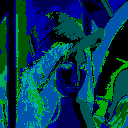
\includegraphics{figures/beelenna.png}} \qquad
  \subfloat[\emph{NDEH}]{\label{fig:lennande}
\includegraphics{figures/ndelenna.png}} \\
  \subfloat[\emph{GAH}]{\label{fig:lennaga}
\includegraphics{figures/galenna.png}} \qquad
  \subfloat[\emph{K-means}]{\label{fig:lennakmeans}
\includegraphics{figures/kmeanslenna.png}} \qquad
  \subfloat[\emph{NPSOH}]{\label{fig:lennapso}
\includegraphics{figures/npsolenna.png}} \\
  \subfloat[\emph{SDEH}]{\label{fig:lennasde}
\includegraphics{figures/sdelenna.png}} \qquad
  \subfloat[\emph{WPSOH}]{\label{fig:lennawpso}
\includegraphics{figures/wpsolenna.png}} \qquad
  \subfloat[Original]{\label{fig:lennaoriginal}
\includegraphics{figures/lenamini.png}} 
  \caption{Mejores soluciones encontradas para \textbf{Lenna}}
  \label{fig:lennaresults}
\end{figure}

\subsection{Comparación por la calidad de solución final: cuantificación del error $J_e$}

    Como se mencionó en la sección \ref{sect:tval}, la cuantificación del error
$J_e$ mide la calidad de una partición en función de la dispersión dentro de los
clusters de la misma. Mientras menor sea el valor de este error, se tiene mejor
calidad de partición.

\subsubsection{Prueba de diferencia de medias}\label{analisis:je_mean_hip}

    Para corroborar los resultados obtenidos en la sección \ref{analisis:db}, se
realizó una prueba de hipótesis de diferencia de medias para la cuantificación
del error $J_e$. Se debe probar para cada par de algoritmos $i, j \in Algorithms
\land i \neq j$ alguna de las siguientes hipótesis:
\begin{itemize}
    \item \emph{Hipótesis nula}: $\bar{X}_i - \bar{X}_j = 0$
    \item \emph{Hipótesis altenativa}: $\bar{X}_i - \bar{X}_j \neq 0$
\end{itemize}
\newpage
donde
\begin{itemize}
    \item $\bar{X}_i$ es la media de las observaciones del valor del error $J_e$
          para el algoritmo $i$.
    \item $Algorithms$ es el conjunto de grupos a estudiar (ver sección
          \ref{analisis:db_mean_hip}).
\end{itemize}

\subsubsection{Prueba de diferencia de varianzas}\label{analisis:je_var_hip}

    Para determinar el estadístico de la prueba descrita en la sección
anterior (ver sección \ref{analisis:je_mean_hip}) es necesario saber si las
observaciones de los valores del error $J_e$ de los di\-fe\-ren\-tes algoritmos
presentan homocedasticidad o heterocedasticidad (igual o diferente varianza
respectivamente). Al igual que en la sección \ref{analisis:db_var_hip}, fue
elegida la prueba de \emph{Levene} \cite{Levene_Test} debido a que permite la
comparación de varianzas de multiples grupos al mismo tiempo. Para esta prueba
se debe probar alguna de las siguientes hipótesis:
\begin{itemize}
    \item \emph{Hipótesis nula}: $\sigma_1 = \sigma_2 = \cdots = \sigma_i = \cdots = \sigma_n$
    \item \emph{Hipótesis alternativa}: al menos una de las varianzas es diferente.
\end{itemize}
donde $\sigma_i$ es la varianza poblacional del error $J_e$ para el algoritmo
$i \in Algorithms$. El estadístico de la prueba de \emph{Levene} está definido
por la ecuación (\ref{levene_est}).

    Como se puede observar en el Resultado \ref{r_je_var_img} se rechaza la hipótesis
nula con un nivel de significancia menor a 5 \% (\emph{p-valor} $ = 3.116 \cdot 10^{-5}$).
Esto significa que existe una diferencia entre las varianzas del error $J_e$
de las muestras de los algoritmos pertenecientes al conjunto $Algorithms$.
\textbf{Por lo tanto, las diferentes muestras presentan heterocedasticidad para
el error $J_e$}.

\begin{lstlisting}[float=h!, caption={Diferencia de Varianza: Cuantificación del error Je}, label=r_je_var_img]
> leveneTest(je, name)
Levene's Test for Homogeneity of Variance (center = median)
       Df F value    Pr(>F)    
group   7  4.9485 3.116e-05 ***
      231                      
---
Signif. codes:  0 '***' 0.001 '**' 0.01 '*' 0.05 '.' 0.1 ' ' 1 
\end{lstlisting}

\subsubsection{Intervalo de confianza de la prueba de diferencia de medias}\label{analisis:je_mean_est}

    En la sección anterior (ver sección \ref{analisis:je_var_hip}), se demostró
que las varianzas de las muestras del error $J_e$ de los algoritmos pertenecientes
al conjunto $Algorithms$ son diferentes. Por lo tanto, el estadístico de la
prueba de hipótesis descrita en la sección \label{analisis:je_mean_hip} no debe
ser sensible a la varianza.

    Sobre los resultados, se aplicó la prueba de \emph{Dunnett-Tukey-Kramer}, también
aplicada sobre las observaciones del índice $DB$ de los diferentes algoritmos
(ver sección \ref{analisis:db_mean_est}).

    En la figura \subref{fig:comp_inter_je}, se pueden observar los intervalos de
confianza de la prueba \emph{T3} para el error $J_e$ de cada algoritmo con los
demás. Los intervalos en rojo indican que existe una diferencia de calidad de las
soluciones finales de los algoritmos comparados con un nivel de significancia de
5 \%. Por otro lado, los intervalos en negro indican que no existe una diferencia
de la calidad de las soluciones de los algoritmos comparados con un nivel de 
significancia de 5 \%.

    De acuerdo a los intervalos de confianza mostrados en la figura
\subref{fig:comp_inter_je} y el diagrama de cajas que aparece en la figura
\subref{fig:comp_je}, se puede concluir que el mejor algoritmo es la
metaheurística \emph{AntH} ya que, en promedio, es diferente a los demás algoritmos
y su error $J_e$ es el más bajo. Sin embargo, esta es la única metaheurística
implementada que no logra definir de manera correcta los clusters de los archivos
de datos probados (\textbf{Lenna} e \textbf{Iris}), como se puede observar la
figura \subref{fig:lennaant}, donde la imagen resultante es difusa.

    El error $J_e$ es bajo para la metaheurística \emph{AntH} ya que ésta no
termina de agrupar los datos, dejando una gran cantidad de patrones dispersos en
clusters pequeños. Esto hace que la cuantificación del error $J_e$ sea ineficaz
para evaluar la verdadera calidad de la partición.

    \textbf{Se puede concluir entonces que el índice $DB$ es más confiable para
medir la calidad de una partición que la cuantificación del error $J_e$.}

\begin{figure}[h!]
  \centering
  \subfloat[\emph{Diagramas de cajas del error $J_e$}]{\label{fig:comp_je}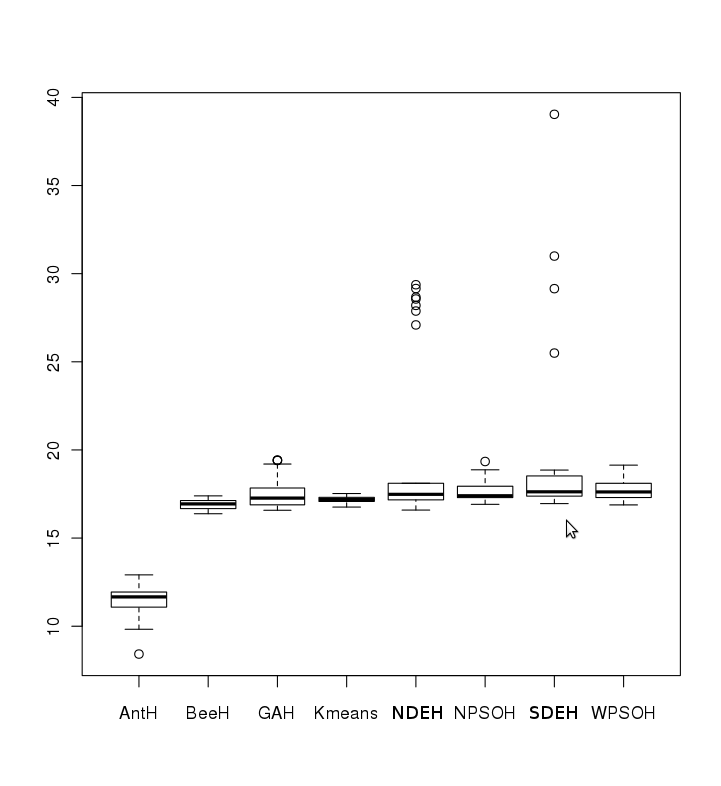
\includegraphics[width=0.6\textwidth]{figures/comp_je.png}}\\
  \subfloat[\emph{Intervalos de confianza del error $J_e$}]{\label{fig:comp_inter_je}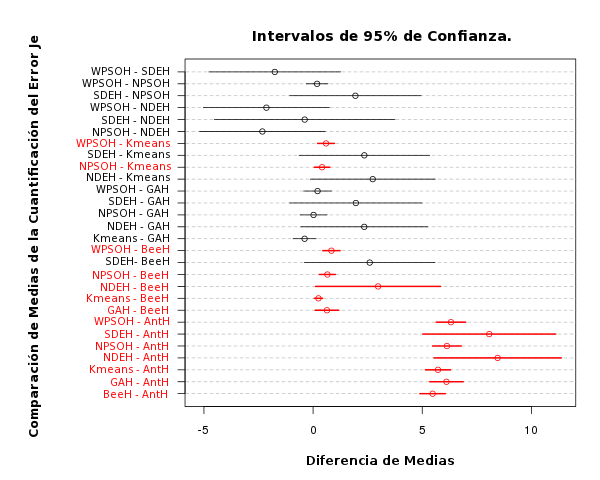
\includegraphics[width=0.6\textwidth]{figures/best_img_je.png}}
  \caption{Comparación del error $J_e$ para \textbf{Lenna}}
  \label{fig:alg_comp_lenna_je}
\end{figure}

\subsection{Comparación de \emph{GAH} y \emph{BeeH} en rendimiento}

    En la sección \ref{analisis:db}, se demostró que las metaheurísticas con 
mejor calidad en sus soluciones finales son \emph{GAH} y \emph{BeeH}. Sin
embargo, estas soluciones son estadísticamente similares, como se demostró en la
sección \ref{analisis:db_mean_est}, y por esto es necesario diferenciarlas
en rendimiento.

    Se utilizó la cantidad de evaluaciones de la función de \emph{fitness}
para comparar a las metaheurísticas \emph{GAH} y \emph{BeeH} porque es una
medida más justa que el tiempo de ejecución. La función de \emph{fitness} es la
función más costosa en tiempo de una metaheurística y la cantidad de veces que es
evaluada durante la ejecución es una cota inferior del tiempo total que pueda
tardar en ejecutarse. Esta medida es independiente del equipo y realmente
refleja el rendimiento de una metaheurística. Como ambas metaheurísticas usan la
misma función de \emph{fitness} para evaluar la calidad de sus soluciones (ver
capítulo \ref{sect:impresultados}), se estudió la cantidad de evaluaciones que
hacen \emph{GAH} y \emph{BeeH} de la misma, para determinar diferencias en el
rendimiento de estos algoritmos (ver apéndice \ref{apendicea}).

\subsubsection{Prueba de diferencia de medias}\label{analisis:eval_mean_hip}

    Se realizó una prueba de hipótesis de diferencia de medias para la cantidad
de evaluaciones de la función de \emph{fitness} de las metaheurísticas \emph{GAH}
y \emph{BeeH}. Se debe probar alguna de las siguientes hipótesis:
\begin{itemize}
    \item \emph{Hipótesis nula}: $\bar{X}_{GAH} - \bar{X}_{BeeH} = 0$
    \item \emph{Hipótesis altenativa}: $\bar{X}_{GAH} - \bar{X}_{BeeH} \neq 0$
\end{itemize}
donde $\bar{X}_{GAH}$ y $\bar{X}_{BeeH}$ son las medias muestrales de la
cantidad de evaluaciones de la función de \emph{fitness} de las metaheurísticas
\emph{GAH} y \emph{BeeH} respectivamente.
\newpage
    Para esto se utilizó la prueba $t$ de \emph{Welch} \cite{AB_0} la cual fue
elegida por no ser sensible a la varianza de los datos. El estadístico de la
prueba es como sigue:

\begin{equation}
    t = \displaystyle\frac{\bar{X}_{GAH} - \bar{X}_{BeeH}}{\sqrt{\frac{S_{GAH}^2}{n_{GAH}} + \frac{S_{BeeH}^2}{n_{BeeH}}}} \sim t_{\nu}
\end{equation}
donde,
\begin{itemize}
    \item $S_{GAH}$ y $S_{BeeH}$ son las varianzas muestrales para \emph{GAH} y
\emph{BeeH} respectivamente.
    \item $n_{GAH}$ y $n_{BeeH}$ son los tamaños de las muestras de \emph{GAH} y
\emph{BeeH} respectivamente.
    \item $\nu$ son los grados de libertad del estadístico y viene dado por la
          ecuación (\ref{eq: nu}) (ver sección \ref{analisis:db_mean_est}).
\end{itemize}

    Como se puede observar en el Resultado \ref{ga_bee_eval_img}, existe una
diferencia en la cantidad de evaluaciones de la función de \emph{fitness} de
ambas metaheurísticas con un nivel de significancia menor a 5 \%
(\emph{p-valor} $= 7.621 \cdot 10^{-16}$). Como la media de la metaheurística \emph{GAH}
($\bar{X}_{GAH} = 35.2069$) es estadísticamente menor que la de \emph{BeeH}
($\bar{X}_{BeeH} = 342.3333$), \emph{GAH} tiene mejor rendimiento que \emph{BeeH}.
\textbf{Por lo tanto, \emph{GAH} es la mejor de las metaheurísticas implementadas
para resolución del problema de \emph{data-clustering} con imágenes.}

\begin{lstlisting}[float=h!, caption={Diferencia de Medias: Evaluaciones de la función de \emph{fitness}}, label=ga_bee_eval_img]
> t.test(eval ~ name)

    Welch Two Sample t-test

data:  eval by name 
t = 15.6604, df = 29.533, p-value = 7.621e-16
alternative hypothesis: true difference in means is not equal to 0 
95 percent confidence interval:
 267.0475 347.2053 
sample estimates:
mean in group BeeH  mean in group GAH 
          342.3333            35.2069
\end{lstlisting}

\subsection{Prueba de la entonación con la imagen sintética}

    Para probar que la entonación de los parámetros de cada metaheurística fue
exitosa, se utilizó la imagen sintética mostrada en la figura \ref{fig:Trivial}
de la sección \ref{datatest}. Esta imagen tiene 7 clusters (6 formas geométricas
y el fondo).

    Como se puede observar en la figura \ref{fig:trivialresults}, todos los
algoritmos logran encontrar los 7 clusters, exceptuando la metaheurística
\emph{AntH}. En la figura \subref{fig:trivialant}, se puede observar algo de
ruido alrededor de algunas de las formas geométricas (puntos de colores),
demostrando que la metaheurística \emph{AntH} fue incapaz de ubicar algunos
patrones (pixeles) en los clusters donde les correspondía.

\begin{figure}[h!]
  \centering
  \subfloat[\emph{AntH}]{\label{fig:trivialant}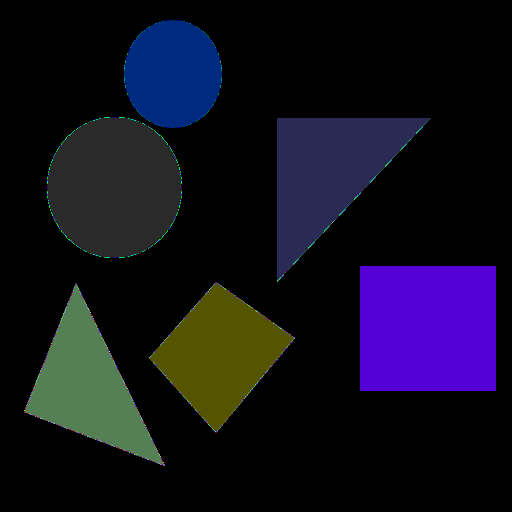
\includegraphics[scale=0.25]{figures/anttrivial.png}} \qquad
  \subfloat[\emph{BeeH}]{\label{fig:trivialbee}
\includegraphics[scale=0.25]{figures/beetrivial.png}} \qquad
  \subfloat[\emph{NDEH}]{\label{fig:trivialnde}
\includegraphics[scale=0.25]{figures/ndetrivial.png}} \\
  \subfloat[\emph{GAH}]{\label{fig:trivialga}
\includegraphics[scale=0.25]{figures/gatrivial.png}}  \qquad
  \subfloat[\emph{K-means}]{\label{fig:trivialkmeans}
\includegraphics[scale=0.25]{figures/kmeanstrivial.png}}  \qquad
  \subfloat[\emph{NPSOH}]{\label{fig:trivialpso}
\includegraphics[scale=0.25]{figures/npsotrivial.png}} \\
  \subfloat[\emph{SDEH}]{\label{fig:trivialsde}
\includegraphics[scale=0.25]{figures/sdetrivial.png}}  \qquad
  \subfloat[\emph{WPSOH}]{\label{fig:trivialwpso}
\includegraphics[scale=0.25]{figures/wpsotrivial.png}}  \qquad
  \subfloat[Original]{\label{fig:trivialoriginal}
\includegraphics[scale=0.25]{figures/trivial.png}}
  \caption{Mejores soluciones encontradas para la imagen sintética}
  \label{fig:trivialresults}
\end{figure}

\section{Análisis de los resultados obtenidos con \emph{Iris}}\label{sect:arcsv}

    A continuación, se presenta un análisis comparativo (similar al hecho para la
imagen \textbf{Lenna}) entre todas las metaheurísticas hibridas implementadas
(\emph{GAH}, \emph{NPSOH}, \emph{WPSOH}, \emph{NDEH}, \emph{SDEH}, \emph{BeeH} y
\emph{AntH}) y el algoritmo determinista \emph{K-means}. Las metaheurísticas
híbridas fueron elegidas para este análisis por presentar mejor calidad en sus
soluciones finales que las metaheurísticas no híbridas (véase el apéndice
\ref{apendicec}).
    Los datos utilizados provienen de los resultados obtenidos con el mejor
conjunto de valores encontrado para cada metaheurística con el archivo de datos
numéricos \textbf{Iris} (ver sección \ref{sect:impresultados} y apéndice
\ref{apendicea}).

\subsubsection{Prueba de diferencia de medias}\label{analisis:db_mean_hip_csv}

    Para determinar diferencias en la calidad de las soluciones finales de los
algoritmos implementados y elegir al mejor de todos, se realizó una prueba de
hipótesis de diferencia de medias para el índice $DB$. Se debe probar para
cada par de algoritmos $i, j \in Algorithms \land i \neq j$ alguna de las
siguientes hipótesis:
\begin{itemize}
    \item \emph{Hipótesis nula}: $\bar{X}_i - \bar{X}_j = 0$
    \item \emph{Hipótesis altenativa}: $\bar{X}_i - \bar{X}_j \neq 0$
\end{itemize}
donde
\begin{itemize}
    \item $\bar{X}_i$ es la media de las observaciones del valor del índice $DB$
          para el algoritmo $i$.
    \item $Algorithms$ es el conjunto de grupos a estudiar (ver sección
          \ref{analisis:db_mean_hip}).
\end{itemize}

    Al igual que en la sección \ref{analisis:db_var_hip}, se realizó una prueba
de hipótesis de \emph{Levene} para determinar diferencia en las varianzas de los
datos. Como se puede observar en el Resultado \ref{r_db_var_csv} existe una diferencia
entre las varianzas del índice $DB$ de los diferentes grupos con un nivel de
significancia menor a 5 \% (\emph{p-valor} $ = 1.636 \cdot 10^{-15}$). \textbf{Por lo tanto,
las diferentes muestras presentan heterocedasticidad}.

\begin{lstlisting}[float=h!, caption={Diferencia de Varianza: Índice \emph{DB}}, label=r_db_var_csv]
> leveneTest(db, name)
Levene's Test for Homogeneity of Variance (center = median)
       Df F value    Pr(>F)    
group   7  14.692 1.636e-15 ***
      208                      
---
Signif. codes:  0 '***' 0.001 '**' 0.01 '*' 0.05 '.' 0.1 ' ' 1
\end{lstlisting}

    Debido a que las muestras presentan varianzas diferentes, se aplicó la prueba
\emph{T3} (ver sección \ref{analisis:db_mean_est}).

    En la figura \subref{fig:comp_inter_csv}, se puede observar los intervalos de
confianza de la prueba \emph{T3} para el índice $DB$ de cada algoritmo con los
demás. Los intervalos en rojo indican que existe una diferencia de calidad de las
soluciones finales de los algoritmos comparados con un nivel de significancia de
5 \%. Por otra lado, los intervalos en negro indican que no existe una diferencia
de la calidad de las soluciones de los algoritmos comparados con un nivel de 
significancia de 5 \%. Los resultados, son similares a los obtenidos en la
sección \ref{analisis:db_mean_est}. Sin embargo, se puede observar que para
\textbf{Iris}, las metaheurísticas \emph{GAH} y \emph{BeeH} presentan calidades
de soluciones finales estadísticamente diferentes. Al observar, además, el
diagrama de cajas presentado en la figura \subref{fig:comp_db_csv}, se puede
concluir que \textbf{\emph{GAH} es la metaheurística con mejor calidad en sus
soluciones finales con respecto a los demás algoritmos comparados, debido a que
su índice $DB$ es estadísticamente el más bajo.}

\begin{figure}[h!]
  \centering
  \subfloat[\emph{Diagramas de cajas del índice $DB$}]{\label{fig:comp_db_csv}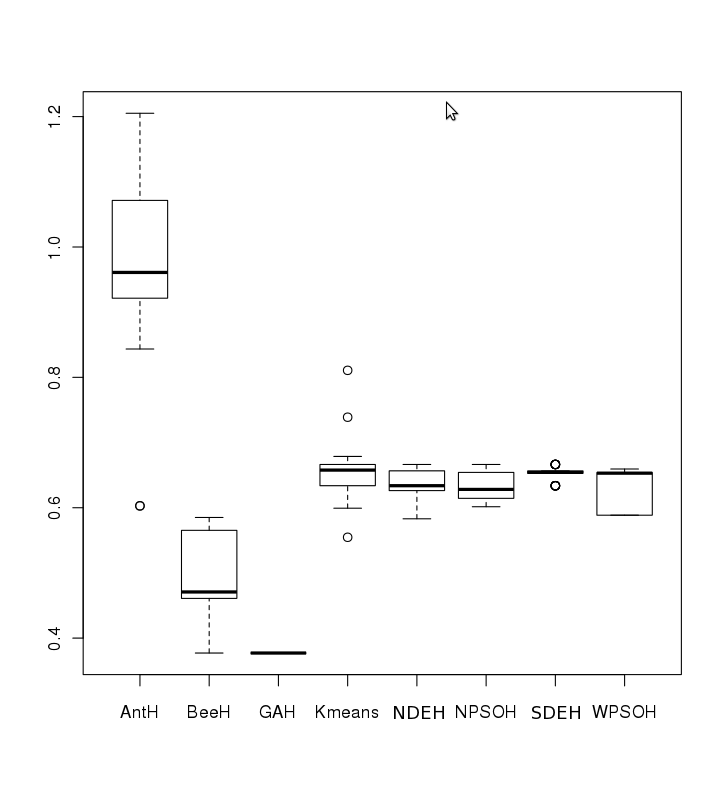
\includegraphics[width=0.6\textwidth]{figures/comp_db_csv.png}}\\
  \subfloat[\emph{Intervalos de confianza del índice $DB$}]{\label{fig:comp_inter_csv}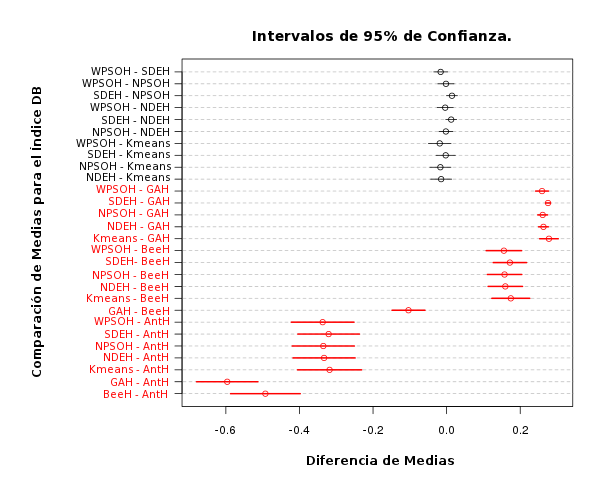
\includegraphics[width=0.6\textwidth]{figures/best_csv_db.png}}
  \caption{Comparación del índice $DB$ para \textbf{Iris}}
  \label{fig:alg_comp_lenna}
\end{figure}
\begin{comment}
\subsection{Imagen sintética}

    Una buena metaheurística sería capaz de particionar correctamente la imagen
sintética. Por lo tanto, fue usada para probar que se realizó una buena
entonación de los parámetros de cada metaheurística. Para más información de la
entonación de los parámetros, véase el apéndice \ref{apendicea}.

    En las figura \ref{fig:trivialresults} se pueden observar los resultados
de cada metaheurística para la imagen sintética. Todas éstas encontraron la
partición óptima para la imagen, exceptuando el \emph{Ant} que tiene ruido
(puntos de muchos colores) en los bordes de algunas de las formas geométricas.
Este ruido implica que la metaheurística \emph{Ant} fue incapaz de ubicar algunos
patrones (píxeles) en los clusters donde les correspondía.

\subsection{\textbf{Lenna}}

    A continuación, se presenta una tabla comparativa de los valores de los
índices de validez de las diferentes metaheurísticas implementadas. Los índices
reportados son los de las mejores soluciones de cada una de éstas para
\emph{Lenna}:

\begin{table}[H]
\footnotesize
\begin{center}
\begin{tabular}{|c|c|c|c|c|c|c|c|c|}
\hline
 & \emph{Ant} & \emph{Bee} & \emph{NDE} & \emph{GA} & \emph{K-means} & \emph{NPSO} & \emph{SDE} & \emph{WPSO} \\
\hline
{\bf DB} & 0.8323    & 0.734   & 0.7493 & 0.709   & 0.7814  & 0.7711  & 0.7578  & 0.7669 \\
\hline
$J_e$    & 11.2246   & 16.9922 & 16.589 & 19.4009 & 16.9164 & 17.3749 & 16.9559 & 16.9839 \\
\hline
{\bf EH} & 100160603 & 284     & 447    & 38      & 7       & 220     & 115     & 183     \\
\hline
\end{tabular}
\caption{Tabla comparativa de las metaheurísticas para {\bf Lenna}}
\label{tb:tableresimg}
\end{center}
\end{table}

    De la tabla \ref{tb:tableresimg} mostrada anteriormente, las gráficas
\ref{fig:alg_comp_lenna} y los resultados para \emph{Lenna} (figura
\ref{fig:lennaresults}), se puede apreciar:

\begin{itemize}
    \item A pesar que la metaheurística \emph{Ant} tiene el menor de los errores
    $J_e$, como se puede ver en la figura \subref{fig:comp_je}, sus soluciones no
    son buenas (ver figura \subref{fig:lennaant}) ya que se obtienen imágenes
    difusas. Esto hace que la cuantificación del error $J_e$ sea ineficaz para
    evaluar la verdadera calidad de la partición.

    El error $J_e$ es bajo para la metaheurística \emph{Ant} ya que ésta no
    termina de agrupar los datos, dejando una gran cantidad de patrones dispersos
    en clusters pequeños.

    \item En la tabla \ref{tb:tableresimg} y el diagrama de cajas \subref{fig:comp_db},
    se puede observar que los valores del índice $DB$ del \emph{Ant} son mayores
    que los de las demás metaheurísticas. Esto significa que es el peor de todos
    los algoritmos al no lograr construir particiones con distancia
     \emph{inter-cluster} alta y distancia \emph{intra-cluster} baja.

    \item En el diagrama \subref{fig:comp_je}, se puede observar un solapamiento
    en las cajas de todas las metaheurísticas, exceptuando el \emph{Ant}, indicando 
    que las medias del error $J_e$ son bastante parecidas entre ellas. Esto
    significa que los algoritmos están construyendo particiones con similar
    dispersión dentro de sus clusters.

    \item En el diagrama \subref{fig:comp_db}, se aprecia que las cajas de las
    metaheurísticas \emph{NDE}, \emph{NPSO}, \emph{SDE} y \emph{WPSO} se solapan,
    indicando que las medias de los valores del $DB$ son similares. Esto puede
    deberse a que comparten el mismo procedimiento que mantiene la cantidad de
    clusters fijos. Además, si comparamos los valores del $DB$ de estas
    metaheurísticas con los de \emph{K-means}, se puede ver que son similares,
    pero tienen mayor valor de \textbf{EH} (véase la tabla \ref{tb:tableresimg}).
    Esto nos permite inferir que estas metaheurísticas no son competitivas con el
    \emph{K-means}.

    \item Sólo las metaheurísticas \emph{Bee} y \emph{GA} muestran valores de
    $DB$ que superan, en promedio, los valores para el algoritmo determinista
    \emph{K-means} (véase diagrama \subref{fig:comp_db}), lo que las hacen ser
    las metaheurísticas de mejor calidad y rendimiento de las implementadas.

    \item En el diagrama \subref{fig:comp_db}, las cajas de los algoritmos
    \emph{Bee} y \emph{GA} se solapan. Esto significa que los valores promedio
    del índice $DB$ son similares y, por ende, ambos consiguen buenas soluciones
    finales por igual. Sin embargo, existen varias diferencias fundamentales
    entre estos dos algoritmos:
    \begin{itemize}
        \item El \emph{GA} no necesita saber de antemano la cantidad total de
        clusters, sino que sólo requiere conocer una cota superior. En cambio, 
        el \emph{Bee} necesita el número de clusters exacto para poder encontrar
        una buena solución.

        \item El \emph{GA} necesita una menor cantidad de evaluaciones promedio
        que el \emph{Bee} lo que la hace una metaheurística más rápida
        (véase diagrama \subref{fig:comp_eval}).
    \end{itemize}
\end{itemize}


\begin{figure}[H]
  \centering
  \subfloat[\emph{Índice $DB$}]{\label{fig:comp_db}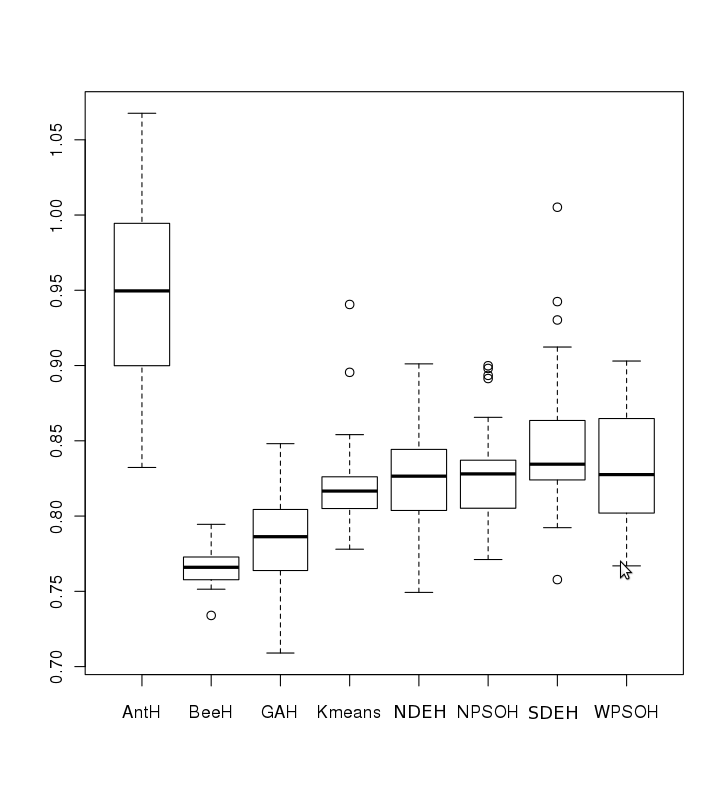
\includegraphics[width=0.5\textwidth]{figures/comp_db.png}}
  \subfloat[\emph{Cuantificación del error $J_e$}]{\label{fig:comp_je}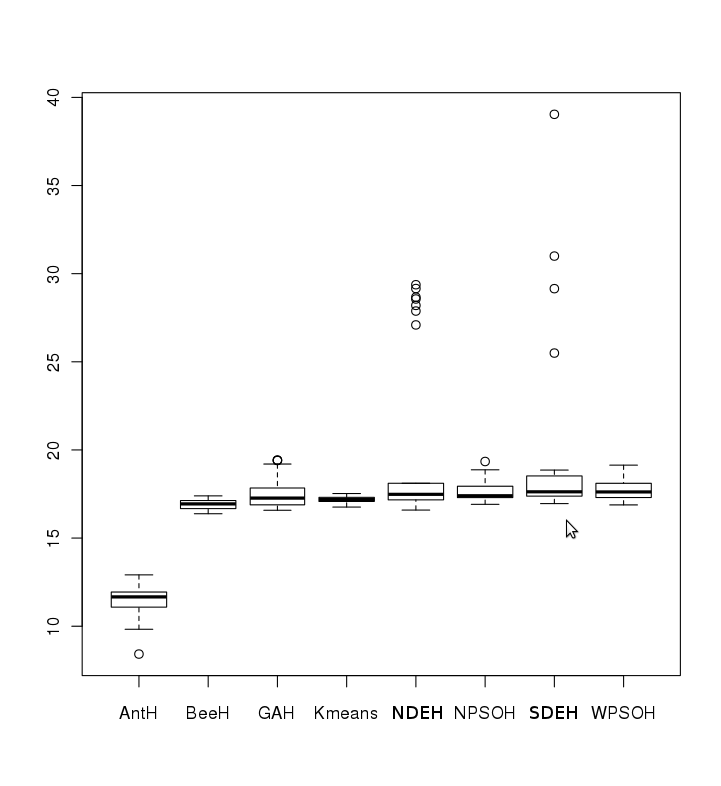
\includegraphics[width=0.5\textwidth]{figures/comp_je.png}}\\
  \subfloat[\emph{Cantidad de evaluaciones totales \textbf{EH}}]{\label{fig:comp_eval}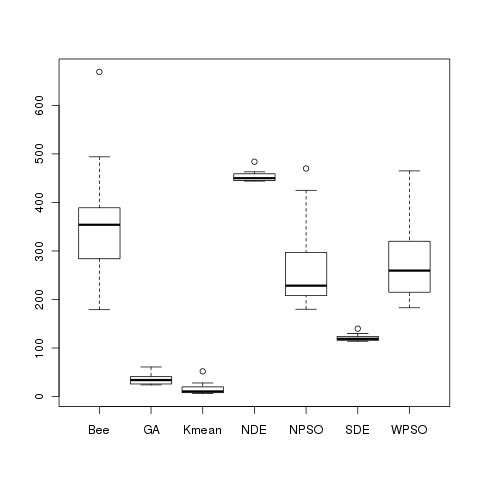
\includegraphics[width=0.5\textwidth]{figures/comp_eval.png}}
  \caption{Diagramas de cajas del $DB$, $J_e$ y \textbf{EH} para \textbf{Lenna}}
  \label{fig:alg_comp_lenna}
\end{figure}

\begin{figure}
  \centering
  \subfloat[\emph{Ant}]{\label{fig:trivialant}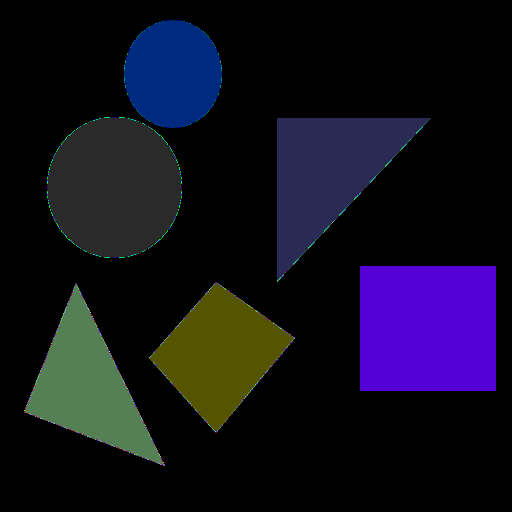
\includegraphics[scale=0.25]{figures/anttrivial.png}} \qquad
  \subfloat[\emph{Bee}]{\label{fig:trivialbee}
\includegraphics[scale=0.25]{figures/beetrivial.png}} \qquad
  \subfloat[\emph{NDE}]{\label{fig:trivialnde}
\includegraphics[scale=0.25]{figures/ndetrivial.png}} \\
  \subfloat[\emph{GA}]{\label{fig:trivialga}
\includegraphics[scale=0.25]{figures/gatrivial.png}}  \qquad
  \subfloat[\emph{K-means}]{\label{fig:trivialkmeans}
\includegraphics[scale=0.25]{figures/kmeanstrivial.png}}  \qquad
  \subfloat[\emph{NPSO}]{\label{fig:trivialpso}
\includegraphics[scale=0.25]{figures/npsotrivial.png}} \\
  \subfloat[\emph{SDE}]{\label{fig:trivialsde}
\includegraphics[scale=0.25]{figures/sdetrivial.png}}  \qquad
  \subfloat[\emph{WPSO}]{\label{fig:trivialwpso}
\includegraphics[scale=0.25]{figures/wpsotrivial.png}}  \qquad
  \subfloat[Original]{\label{fig:trivialoriginal}
\includegraphics[scale=0.25]{figures/trivial.png}}
  \caption{Mejores soluciones encontradas para la imagen sintética}
  \label{fig:trivialresults}
\end{figure}

\begin{figure}
  \centering
  \subfloat[\emph{Ant}]{\label{fig:lennaant}
\includegraphics{figures/antlenna.png}} \qquad
  \subfloat[\emph{Bee}]{\label{fig:lennabee}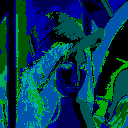
\includegraphics{figures/beelenna.png}} \qquad
  \subfloat[\emph{NDE}]{\label{fig:lennande}
\includegraphics{figures/ndelenna.png}} \\
  \subfloat[\emph{GA}]{\label{fig:lennaga}
\includegraphics{figures/galenna.png}} \qquad
  \subfloat[\emph{K-means}]{\label{fig:lennakmeans}
\includegraphics{figures/kmeanslenna.png}} \qquad
  \subfloat[\emph{NPSO}]{\label{fig:lennapso}
\includegraphics{figures/npsolenna.png}} \\
  \subfloat[\emph{SDE}]{\label{fig:lennasde}
\includegraphics{figures/sdelenna.png}} \qquad
  \subfloat[\emph{WPSO}]{\label{fig:lennawpso}
\includegraphics{figures/wpsolenna.png}} \qquad
  \subfloat[Original]{\label{fig:lennaoriginal}
\includegraphics{figures/lenamini.png}} 
  \caption{Mejores soluciones encontradas para \textbf{Lenna}}
  \label{fig:lennaresults}
\end{figure}

\section{Resultados para \textbf{Iris}}\label{sect:arcsv}

    A continuación, se presenta una tabla comparativa de los valores de los
índices de validez las diferentes metaheurísticas implementadas. Los índices
reportados son los de las mejores soluciones de cada una de éstas para \emph{Iris}:

\begin{table}[h!]
\footnotesize
\begin{center}
\begin{tabular}{|c|c|c|c|c|c|c|c|c|}
\hline
 & \emph{Ant} & \emph{Bee} & \emph{NDE} & \emph{GA} & \emph{K-means} & \emph{NPSO} & \emph{SDE} & \emph{WPSO} \\
\hline
{\bf DB}  & 0.6029  & 0.3771 & 0.583  & 0.3771 & 0.599  & 0.6015 & 0.6338 & 0.5885 \\
\hline
$J_e$     & 0.4881  & 0.5029 & 0.6586 & 0.5029 & 0.6339 & 0.6807 & 0.625  & 0.6709 \\
\hline
{\bf EH}  & 1000163 & 304    & 170    & 47     & 5      & 130    & 171    & 45     \\
\hline
\end{tabular}
\caption{Tabla comparativa de las metaheurísticas para {\bf Iris}}
\label{tb:tablerescsv}
\end{center}
\end{table}

        De la tabla \ref{tb:tablerescsv} mostrada anteriormente y las gráficas
\ref{fig:alg_comp_iris}, se puede llegar a conclusiones similares a las
obtenidas para \textbf{Lenna}. Sin embargo, se pueden apreciar las siguientes
diferencias:
\begin{itemize}
    \item En el diagrama \subref{fig:comp_db_csv}, se puede observar que el
    \emph{GA} tiene mejores valores de índice $DB$, en promedio, que el \emph{Bee},
    No obstante, ambas metaheurísticas siguen superando a las demás.

    \item A diferencia de los resultados para \textbf{Lenna}, las distribuciones
    del error $J_e$ para el \emph{GA} y el \emph{Bee} superan a las de las
    demás metaheurísticas (véase el diagrama \subref{fig:comp_db_csv}).
\end{itemize}

\begin{figure}[H]
  \centering
  \subfloat[\emph{Índice $DB$}]{\label{fig:comp_db_csv}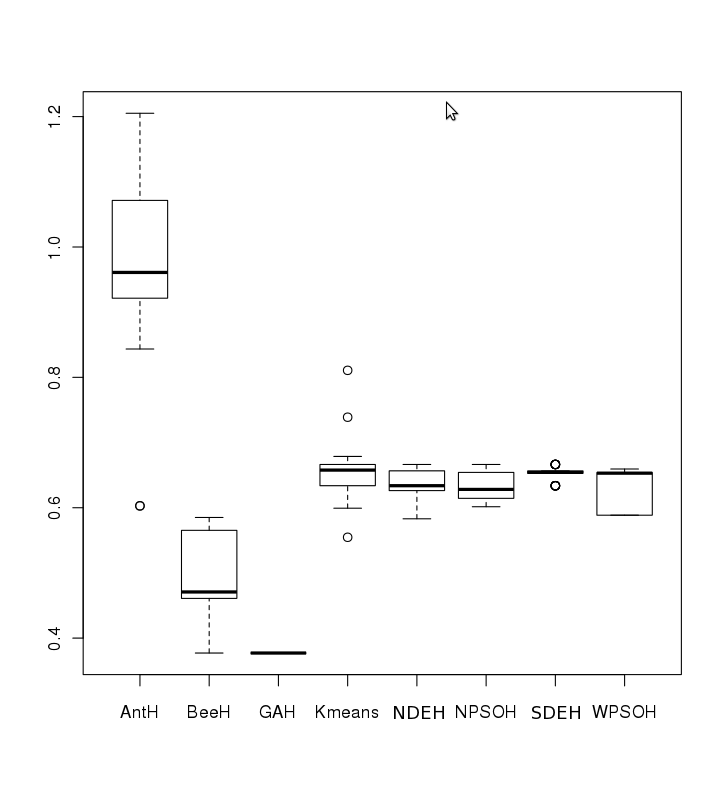
\includegraphics[width=0.5\textwidth]{figures/comp_db_csv.png}}
  \subfloat[\emph{Cuantificación del error $J_e$}]{\label{fig:comp_je_csv}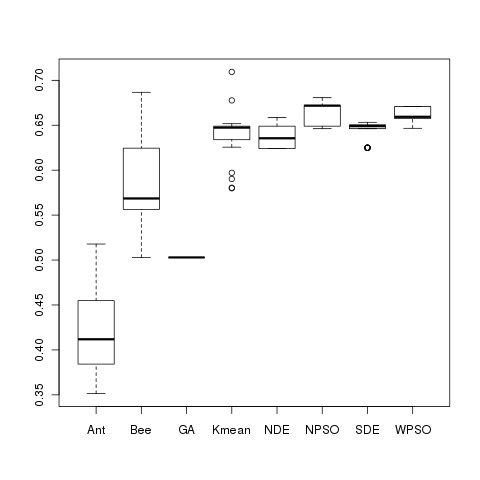
\includegraphics[width=0.5\textwidth]{figures/comp_je_csv.png}}\\
  \subfloat[\emph{Cantidad de evaluaciones totales \textbf{EH}}]{\label{fig:comp_eval_csv}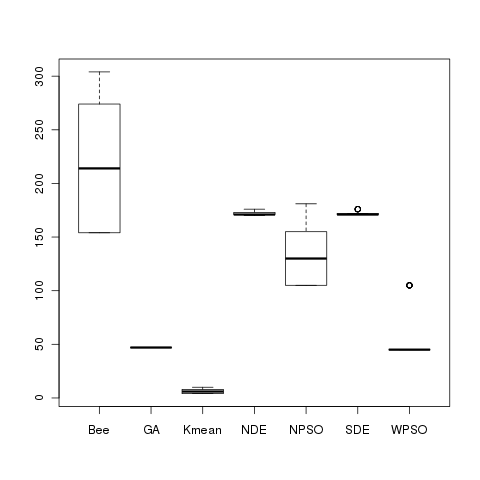
\includegraphics[width=0.5\textwidth]{figures/comp_eval_csv.png}}
  \caption{Diagramas de cajas del $DB$, $J_e$ y \textbf{EH} para \textbf{Iris}}
  \label{fig:alg_comp_iris}
\end{figure}

\end{comment}
